\documentclass[xetex,mathserif,serif]{beamer}
\usepackage{polyglossia}
\setdefaultlanguage[babelshorthands=true]{russian}
\usepackage{minted}
\usepackage{tabu}

\useoutertheme{infolines}

\usepackage{fontspec}
\setmainfont{FreeSans}
\newfontfamily{\russianfonttt}{FreeSans}

\usepackage{textpos}
\setlength{\TPHorizModule}{1cm}
\setlength{\TPVertModule}{1cm}

\setbeamertemplate{blocks}[rounded][shadow=false]

\definecolor{links}{HTML}{2A1B81}
\hypersetup{colorlinks,linkcolor=,urlcolor=links}

\tabulinesep=1.2mm

\title{Программная инженерия, практика}
\subtitle{Занятие 1: Введение}
\author[Юрий Литвинов]{Юрий Литвинов\\\small{\textcolor{gray}{yurii.litvinov@gmail.com}}}
\date{04.09.2019}

\newcommand{\todo}[1] {
	\begin{center}\textcolor{red}{TODO: #1}\end{center}
}

\newcommand{\DownArrow} {
	\hspace{2cm}\begin{LARGE}$\downarrow$\end{LARGE}
}

\begin{document}

	\frame{\titlepage}

	\section{Введение}

	\begin{frame}
		\frametitle{О чём этот курс}
		\begin{itemize}
			\item Средство опробовать на практике знания, полученные из теоретического курса
			\begin{itemize}
				\item Далеко не все
			\end{itemize}
			\item Не будем писать код (ну, почти)
			\begin{itemize}
				\item Курс очень гуманитарный, но увы, это тоже надо уметь
			\end{itemize}
			\item Будем <<разрабатывать>> воображаемые проекты
			\begin{itemize}
				\item Для этого их придётся придумать
			\end{itemize}
			\item Часть заданий будет прямо на паре, часть --- дома
			\item Telegram-группа курса: \url{https://t.me/joinchat/EptgDVdWyEpVlrBlncTVew}
			\item Все материалы курса и задания: \url{http://hwproj.me/courses/45}
		\end{itemize}
	\end{frame}

	\begin{frame}
		\frametitle{Организационное}
		Оценка:
		\begin{itemize}
			\item 50\% --- оценка за экзамен
			\item 40\% --- оценка за коллковиум
			\item 10\% --- оценка за практику (catch в том, что надо сдать всё)
		\end{itemize}
		Практика:
		\begin{itemize}
			\item Домашние работы
			\item Проекты групповые
			\begin{itemize}
				\item Поэтому первая задача --- разбиться на команды
			\end{itemize}
			\item Надо прочитать одну из книг по управлению проектами и написать двухстраничный отзыв к концу курса
		\end{itemize}
	\end{frame}

	\begin{frame}
		\frametitle{Книги}
		\begin{footnotesize}
			\begin{itemize}
				\item \textbf{Роберт Гласс} Программирование и конфликты
				\item \textbf{Т. Питерс} Основы. Лидерство.
				\item \textbf{П.Ф. Друкер} Практика менеджмента
				\item Project Management Body of Knowledge
				\item \textbf{Т. ДеМарко, Т. Листер} Вальсируя с медведями: управление рисками в проектах по разработке программного обеспечения.
				\item \textbf{Т. ДеМарко, Т. Листер} Балдеющие от адреналина и зомбированные шаблонами. Паттерны поведения проектных команд.
				\item \textbf{Т. ДеМарко, Т. Листер} Человеческий фактор. Успешные проекты и команды.
				\item \textbf{Т. ДеМарко} Deadline. Роман об управлении проектами.
				\item \textbf{Ф. Брукс} Мифический человеко-месяц
				\item \textbf{Дж. Рейнвотер} Как пасти котов
				\item \textbf{Э. Хант} Программист-прагматик. Путь от подмастерья к мастеру
				\item \textbf{Дж. Спольски} Джоэл о программировании
				\item \textbf{И. Соммервилл} Инженерия программного обеспечения
				\item ...
			\end{itemize}
		\end{footnotesize}
	\end{frame}

	\begin{frame}
		\frametitle{Что будет в курсе}
		\begin{footnotesize}
			\begin{itemize}
				\item Работа с требованиями
				\item Устав проекта
				\item Практики Agile-методологий (парное программирование, backlog, спринты)
				\item Декомпозиция и дерево задач
				\item Управление рисками
				\item Оценка и слежение за ходом проекта --- диаграммы Гантта, сетевой график
				\item Управление изменениями
				\item Техническое задание
				\item План тестирования
				\item Багтрекинг
				\item CRM (если успеем)
			\end{itemize}
		\end{footnotesize}
	\end{frame}

	\section{Пример проекта}

	\begin{frame}
		\frametitle{Пример проекта}
		Информационный портал студотдела
		\begin{itemize}
			\item Цель проекта:
			\begin{itemize}
				\item автоматизировать выдачу справок об обучении, приём заявлений на повышенную стипендию
			\end{itemize}
			\item Требования:
			\begin{itemize}
				\item облегчать процесс получения справки
				\item облегчать процесс подачи студентами заявлений
				\item снижать нагрузку на работников деканата
				\item клиентская часть должна корректно работать в Google Chrome, Mozilla Firefox, Opera
				\item система должна иметь возможность одновременно работать с не менее 100 запросов без существенных потерь производительности
				\item время обработки одного запроса должно быть не более 5 сек
			\end{itemize}
		\end{itemize}
	\end{frame}

	\begin{frame}
		\frametitle{Диаграмма случаев использования}
		\begin{center}
			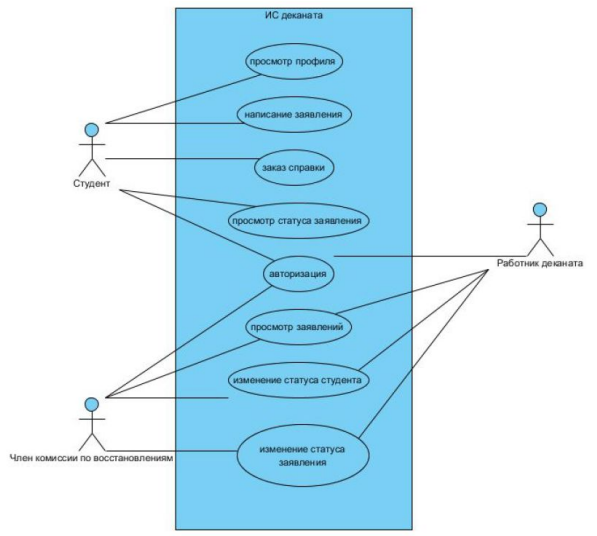
\includegraphics[width=0.6\textwidth]{useCase.png}
		\end{center}
	\end{frame}

	\begin{frame}
		\frametitle{Дерево задач}
		\begin{center}
			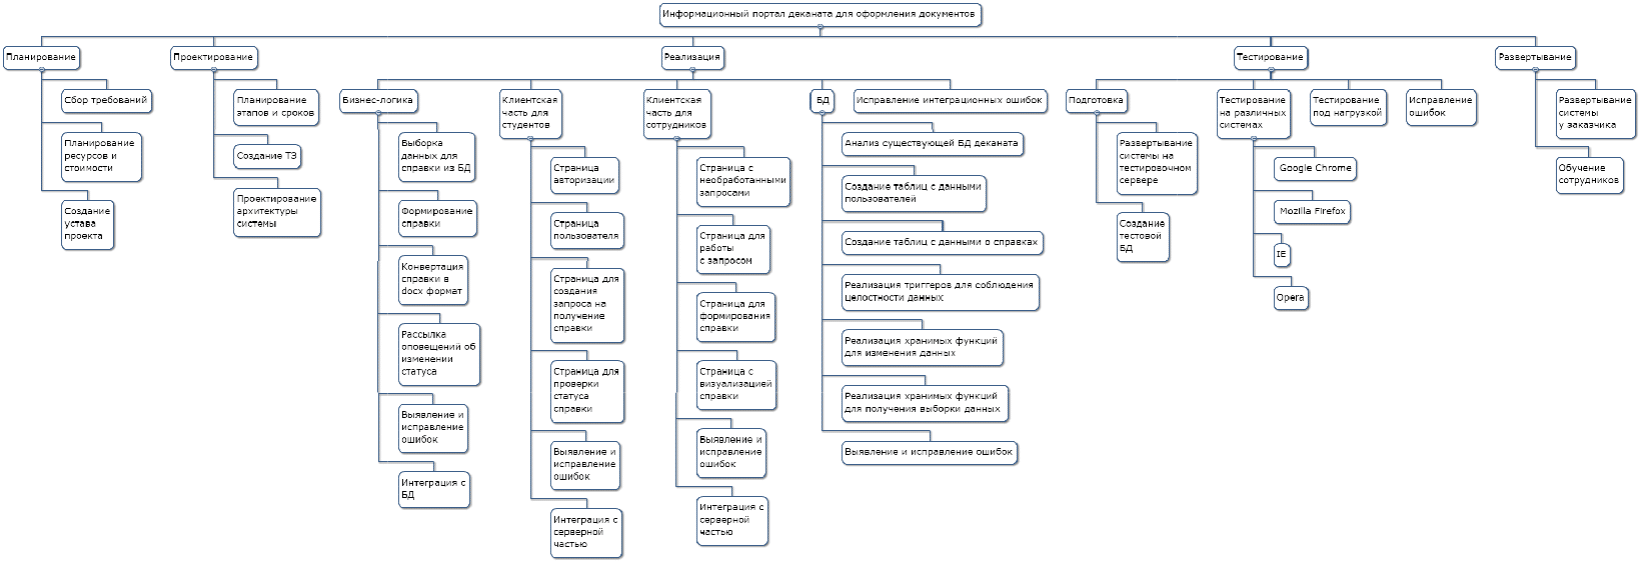
\includegraphics[width=\textwidth]{wbs.png}
		\end{center}
	\end{frame}

	\begin{frame}
		\frametitle{Риски}
		\begin{itemize}
			\item Недостатки планирования
			\begin{itemize}
				\item \textbf{Последствия} --- потеря времени, денег, в случае, если проект будет задержан на очень большое время --- потеря репутации
				\item \textbf{Вероятность} --- высокая
				\item \textbf{Угроза} --- высокая
				\item \textbf{Меры предотвращения} --- заложить дополнительно 80\% к времени и ресурсам, пригласить опытного специалиста для оценки проекта
			\end{itemize}
			\item Текучка кадров
			\begin{itemize}
				\item \textbf{Последствия} --- увеличение требуемого времени
				\item \textbf{Вероятность} --- высокая
				\item \textbf{Угроза} --- высокая
				\item \textbf{Меры предотвращения} --- попытаться найти средства для финансирования проекта, предложить участникам темы курсовых/дипломных работ в проекте
			\end{itemize}
			\item ...
		\end{itemize}
	\end{frame}

	\begin{frame}
		\frametitle{План проекта}
		\begin{center}
			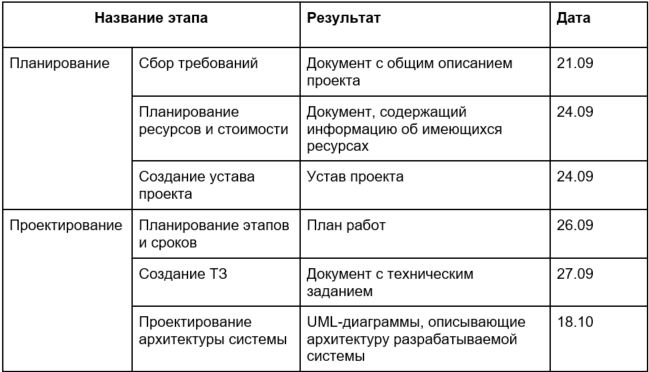
\includegraphics[width=0.8\textwidth]{plan1.png}
		\end{center}
	\end{frame}

	\begin{frame}
		\frametitle{План проекта (2)}
		\begin{center}
			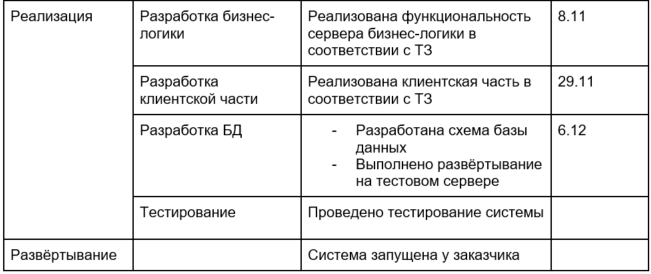
\includegraphics[width=0.8\textwidth]{plan2.png}
		\end{center}
	\end{frame}

	\begin{frame}
		\frametitle{Диаграмма Гантта}
		\begin{center}
			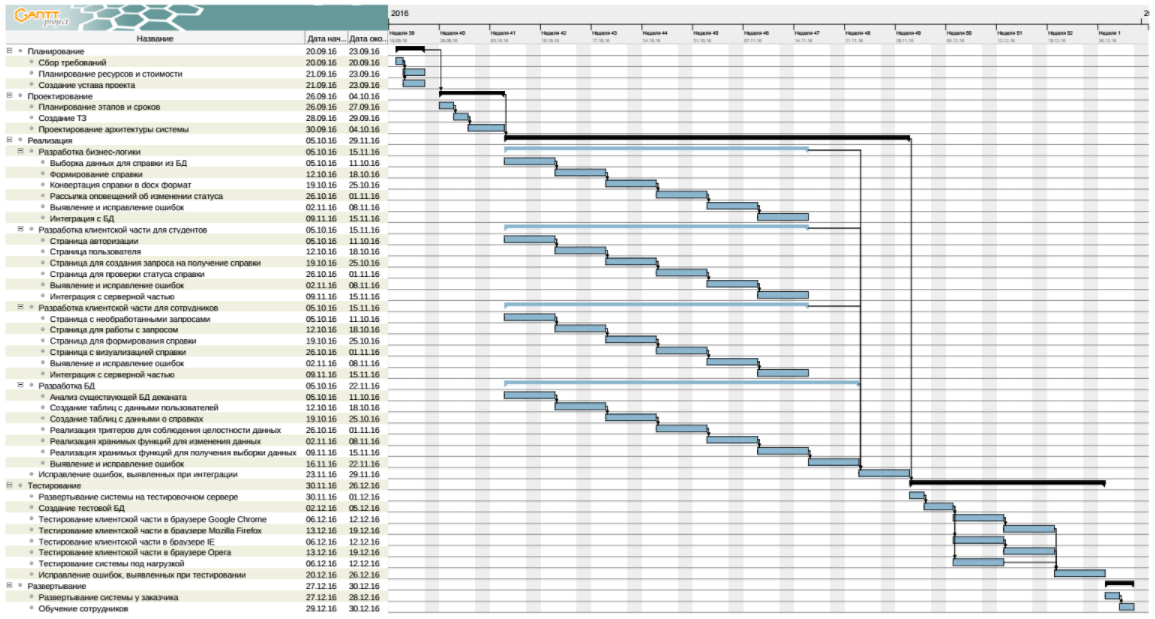
\includegraphics[width=\textwidth]{ganttChart.png}
		\end{center}
	\end{frame}

	\begin{frame}
		\frametitle{Описание вакансии}
		\begin{scriptsize}
			Молодая и успешная команда ищет разработчика C\# для создания и оптимизации кода серверной части информационной системы студотдела.

			Мы разрабатываем современный программный продукт, который поможет облегчить взаимодействие студентов и студотдела ВШЭ.

			Требования к кандидату:
			\begin{itemize}
				\item глубокое знание возможностей языка С\# и платформы .NET;
				\item понимание принципов разработки на ASP.NET;
				\item ...
			\end{itemize}

			Преимуществом будет:
			\begin{itemize}
				\item опыт работы с AngularJS, HTML5, CSS3, JavaScript, jQuery;
				\item ...
			\end{itemize}

			Обязанности:
			\begin{itemize}
				\item разработка сложной бизнес-логики;
				\item ...
			\end{itemize}

			Условия:
			\begin{itemize}
				\item использование в работе передовых технологий;
				\item возможность забить и не работать вообще.
			\end{itemize}
		\end{scriptsize}
	\end{frame}

	\begin{frame}
		\frametitle{План собеседования}
		\begin{small}
			\begin{itemize}
				\item Поздороваться
				\item Сказать, что экзаменатора пока нет, и что мне сказали сюда прийти встретить его и я просто его возможный будущий коллега
				\item \textbf{Коммуникабельность, поведенческие качества} --- завести дежурный разговор: спросить из какого он вуза, кафедры, если из АУ, то спросить, кого он выбрал в научные руководители
				\item Далее получить сообщение (от себя же), что интервьюер не придёт, и что мне нужно самому провести собеседование
				\item \textbf{Технические навыки}
				\begin{itemize}
					\item ​Когда вызываются статические конструкторы классов в C\#?
					\item Каким образом можно перехватить добавление и удаление делегата из события?
					\item Попросить объяснить принцип работы git
				\end{itemize}
				\item \textbf{Прошлый опыт} --- спросить, в каких проектах он до этого участвовал, в чём заключалась его конкретная задача
				\item ...
			\end{itemize}
		\end{small}
	\end{frame}

	\section{Домашнее задание}

	\begin{frame}
		\frametitle{Домашнее задание}
		\begin{itemize}
			\item Разделиться на команды по 3 человека
			\item Придумать проект, для которого будете писать документацию
			\begin{itemize}
				\item Это может быть ваша НИР, ваша прошлая НИР или вообще выдуманный с нуля проект
				\item Он должен быть достаточно содержателен, хотя бы на пару человеколет работы
				\item Реализовывать его будет не нужно
				\item Самые подходящие проекты будут предложены как учебные практики студентам СПбГУ
			\end{itemize}
			\item Подготовить презентацию на 10 минут с представлением идеи проекта
			\item Дедлайн --- \textbf{11 сентября}
		\end{itemize}
	\end{frame}

\end{document}
